\chapter{Introduction}

\section{Modélisation numérique de la circulation océanique}

La modélisation de la circulation océanique se développe dès les années 1950. Henri Stommel propose en 1948 un premier modèle dynamique du Gulf Stream \cite{stommel_westward_1948}, que Walter Munk améliore deux ans plus tard en y intégrant des effets de dissipation et les interactions avec le vent \cite{munk_wind-driven_1950}. Ces apports permettent une compréhension approfondie des gyres océaniques à grande échelle. Les premiers modèles numériques tridimensionnels de la circulation océanique apparaissent dans les années 1960, sous l’impulsion de Kirk Bryan et Michael Cox \cite{bryan_nonlinear_1968, bryan_nonlinear_1968-1}, avec le développement du modèle \textbf{MOM}.

Depuis les années 1990, les modèles de circulation océanique ont évolué vers des systèmes plus réalistes, prenant en compte de plus en plus de variables, paramétrisations, des échelles plus fines ainsi que des bathymétries réalistes. Parmi les plus utilisés aujourd’hui dans la recherche figurent le modèle \textbf{CROCO}, construit autour de \textbf{ROMS} \cite{moore_regional_2011}, et le modèle \textbf{NEMO} \cite{madec_ocean_1997}, qui servent à produire des simulations déterministes de la circulation océanique.

La multiplicité des forçages et paramétrisations, ainsi que la nature chaotique des systèmes océaniques et atmosphériques, qui résolvent les tourbillons de méso-échelle (de l'ordre du rayon de déformation de Rossby), posent cependant un défi aux approches déterministes classiques. Les modèles numériques actuels produisent généralement une seule simulation correspondant à une solution des équations de circulation, négligeant ainsi la variabilité intrinsèque du système. Jusqu’aux années 2010, les limitations informatiques empêchaient la réalisation d’ensembles de simulations permettant d’explorer cette variabilité.

Afin d'explorer et de caractériser cette variabilité, la recherche s’oriente depuis une quinzaine d’années vers les simulations ensemblistes. Des ensembles sont ainsi utilisés pour mettre en oeuvre des approches probabilistes, permettant de représenter explicitement les incertitudes des modèles et d’analyser la dispersion des évolutions possibles du système. Si la variabilité intrinsèque est aujourd'hui de plus en plus explorée, les études probabilistes s'intéressant également à l'impact des perturbations des modèles sur cette variabilité sont moins nombreuses.

\section{Incertitudes dans les systèmes de modélisation}

Les modèles numériques de circulation océanique reposent sur des hypothèses simplificatrices nécessaires pour réduire le coût computationnel. Ces hypothèses, bien que nécessaires, introduisent des incertitudes dans les sorties du modèle, en particulier pour les processus physiques qui ne sont pas explicitement résolus (lié à la résolution de la grille par exemple). Dans le cadre de ce travail, le terme \textit{incertitudes} désignera exclusivement ces incertitudes issues de la modélisation numérique ; lorsqu’il sera question d’incertitudes de mesure, cela sera explicitement précisé.

Ces incertitudes peuvent avoir plusieurs origines. La première est la variabilité intrinsèque, liée au caractère chaotique du système d’équations gouvernant la circulation océanique et qui limite la prédictibilité du système. À cela s’ajoutent les incertitudes liées aux conditions de forçage, qu’il s’agisse des flux atmosphériques appliqués à la surface de l’océan ou des conditions initiales et aux frontières imposées par des données externes. Enfin, les \textit{processus sous-maille}, c’est-à-dire ceux dont l’échelle spatiale est inférieure à la résolution de la grille du modèle, génèrent également des incertitudes qui peuvent devenir significatives selon la configuration utilisée.

Parmi l’ensemble de ces sources, la variabilité intrinsèque est toujours présente. Elle sera donc systématiquement représentée dans les expériences menées dans ce travail. Une analogie peut être faite avec l’attracteur de Lorenz \cite{atencia_analogs_2017}, pour illustrer comment de petites différences initiales peuvent entraîner une divergence marquée entre trajectoires dans un système chaotique.

Les autres sources d’incertitudes se superposent à la variabilité intrinsèque et contribuent à participer à l'augmentation de la dispersion des trajectoires simulées. Dans cette étude, nous nous concentrerons sur deux sources d’incertitudes supplémentaires :
\begin{itemize}
    \item les incertitudes sur les flux turbulents de quantité de mouvement dans le forçage atmosphérique ;
    \item les incertitudes liées à la paramétrisation de la turbulence verticale, notamment dans les modèles GLS (\textit{Generic Length Scale}) utilisés pour modéliser l’énergie cinétique turbulente.
\end{itemize}

\section{Cadre régional d'étude}

La présente étude se focalise sur une région spécifique : l’océan Indien sud-ouest. Cette zone se distingue par des conditions climatiques particulières, influencées par la géographie singulière de l’océan Indien. Contrairement aux océans Atlantique et Pacifique, cet océan est fermé au nord par le continent. De plus, les fortes variations saisonnières climatiques en Asie génèrent des mousson plus conséquente, structurant les saisons sèches et humides dans la région. Cette dynamique entraîne des inversions saisonnières des vents, responsables d’une inversion annuelle des courants, notamment le courant de Somalie et le courant subéquatorial \cite{phillips_progress_2021}, comme illustré dans la \autoref{fig:dynamics}.

\begin{figure}[h]
\centering
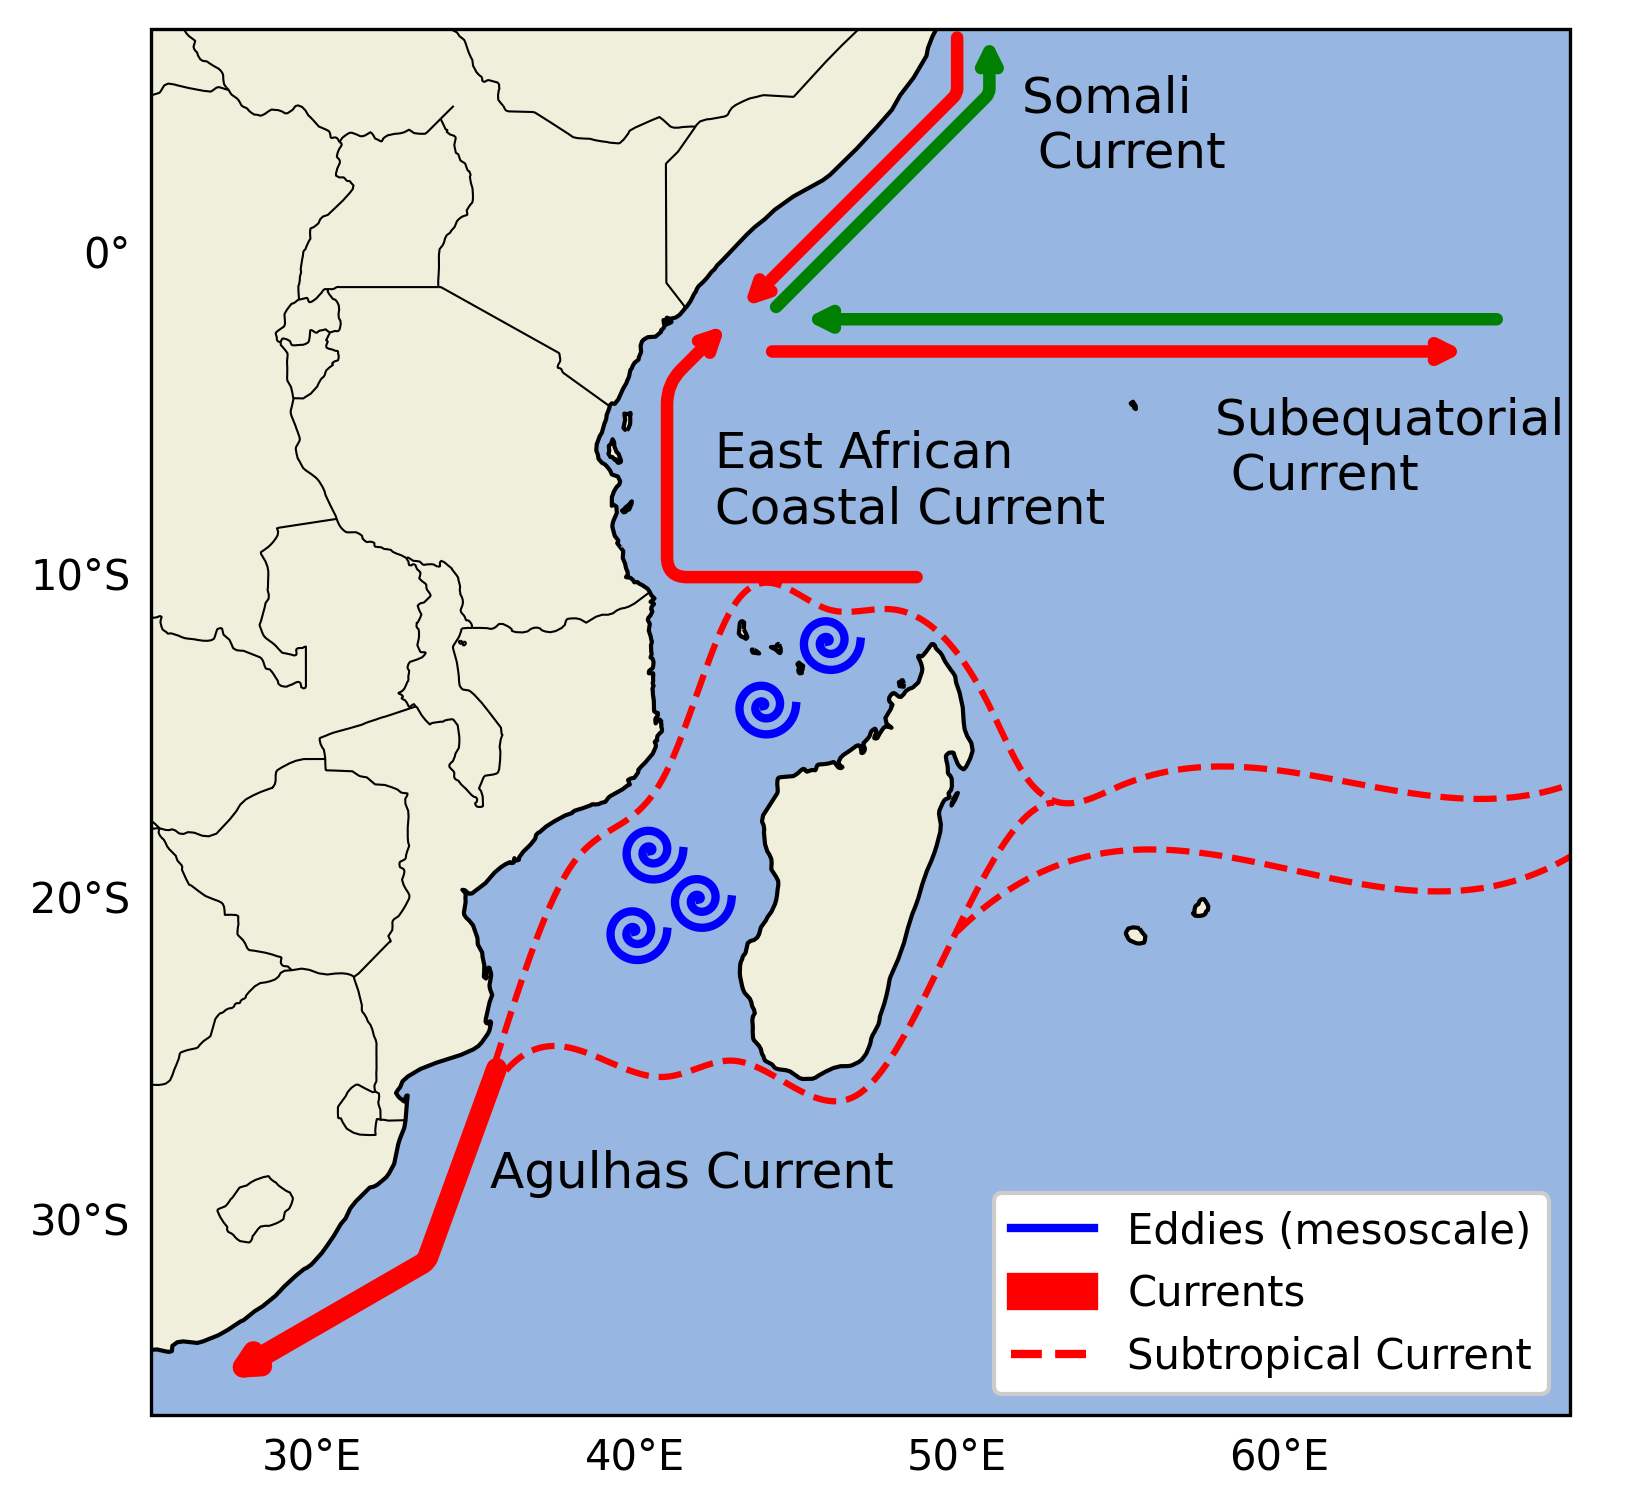
\includegraphics[width=0.6\textwidth]{Figures/dynamics.png}
\caption{Schéma de la dynamique de l’océan Indien sud-ouest, inspiré de \cite{phillips_progress_2021}}
\label{fig:dynamics}
\end{figure}

Outre ces courants de variabilité saisonnière, la région est dominée par deux courants de bord ouest majeurs : le courant des Aiguilles et le courant côtier d’Afrique de l’Est. Ces deux courants ne subissent pas d’inversion au cours de l’année, mais jouent un rôle essentiel dans la dynamique océanique régionale et même globale. Le courant des Aiguilles permet le transfert de chaleur de l’océan Indien vers l’océan Atlantique.

Un autre acteur important de la circulation est le courant subtropical, en provenance de l’Indonésie, qui atteint la côte est de Madagascar. À cet endroit, il se divise en deux jets qui contournent l’île de part et d’autre. Cette interaction bathymétrique est à l’origine de la formation de nombreux tourbillons de méso-échelle, particulièrement présents dans le canal du Mozambique et autour des archipels situés plus au nord, comme Mayotte et les Comores.

Cette dynamique complexe de la circulation océanique entraîne d’importants échanges de particules entre les différentes sous-régions de l’océan Indien sud-ouest. Ces particules peuvent être vivantes (plancton, larves) ou inertes (polluants) \cite{murphy_global_2021}, et circulent entre les archipels, les zones économiques exclusives (ZEE) ou les Aires Marines Protégées (AMP). Ces processus d’échange sont désignés sous le terme de connectivités marines, et représentent une caractéristique clé dans la planification et la gestion de l'espace marin. À l’heure actuelle, ces connectivités sont généralement estimées à l’aide de simulations déterministes ou de réanalyse Mercator \cite{maina_aligning_2020} , ce qui ne permet pas de représenter correctement l'éventail de dispersions induite par les variations fines de la circulation océanique. Dans ce contexte, il est crucial d’intégrer l’incertitude dans ces évaluations, en particulier pour répondre aux objectifs des Nations Unies visant à protéger 30\% des océans par des aires marines protégées d’ici 2030.

\section{Questions de recherche et objectifs scientifiques}

Ce travail s’inscrit dans une démarche visant à transformer un modèle océanique régional, initialement déterministe, en un cadre probabiliste capable de simuler explicitement différentes sources d’incertitudes. L’objectif principal est de diagnostiquer les effets de ces incertitudes sur la circulation océanique simulée. Pour cela, nous avons conçu et mis en œuvre différents ensembles de simulations, chacun intégrant une perturbation ciblée sur un paramètre ou un processus physique particulier, que l'on juge incertain, telle que la tension du vent ou la paramétrisation du mélange vertical. L’analyse comparative de ces ensembles permet de quantifier et de caractériser l’impact de chaque perturbation sur la dynamique du modèle, tout en mettant en lumière le rôle central de la variabilité intrinsèque dans le contrôle de la dispersion des simulations.

Au-delà de cet aspect méthodologique, les simulations produites ont également une finalité appliquée : elles servent à étudier l'effet cumulatif de différentes sources d'incertitudes, comment elles se superposent et interagissent entre elles. De plus ces données servent de travail préparatoire à l'inversion d'observation de courant de surface, notamment pour le calcul de connectivités.





